% ======================================================================
% Auto-generated figure include snippets for LaTeX
% Generated: 2026-06-22
% ======================================================================

% --- Figure 1: Two-layer parser sensitivity ---
\begin{figure*}[htb!]
    \centering
    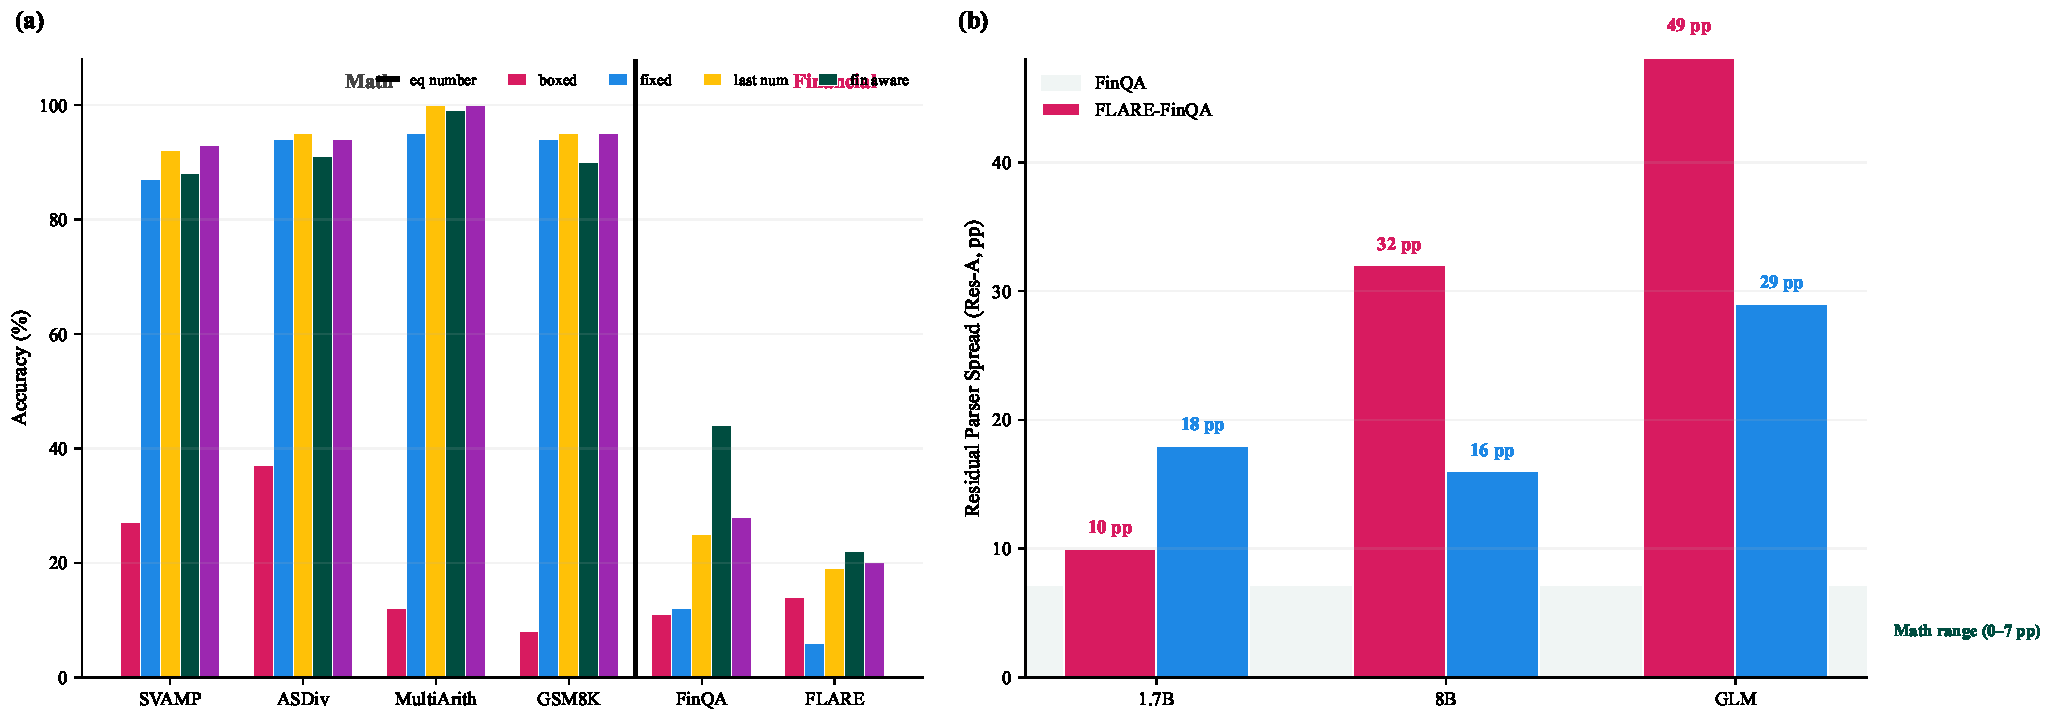
\includegraphics[width=\textwidth]{figures/figure1_two_layer.pdf}
    \caption{%
    Two-layer parser sensitivity.
    (a)~Parser accuracy across four mathematical and two financial benchmarks (Qwen3-8B).
    The domain separator marks the transition from clean-answer math benchmarks to format-diverse financial ones.
    (b)~Residual parser spread (Res-A, excluding \numparser{}) by model scale.
    Financial benchmarks retain 10--39\,pp residual sensitivity, compared to 1--7\,pp on math (shaded region).
    The spread increases with model capacity on FinQA (10\,pp~$\to$~32\,pp~$\to$~38\,pp from 1.7B to 30B), indicating that larger models produce more diverse output formats.}
    \label{fig:two_layer}
\end{figure*}

% --- Figure 2: Best parser by benchmark and model ---
\begin{figure*}[htb!]
    \centering
    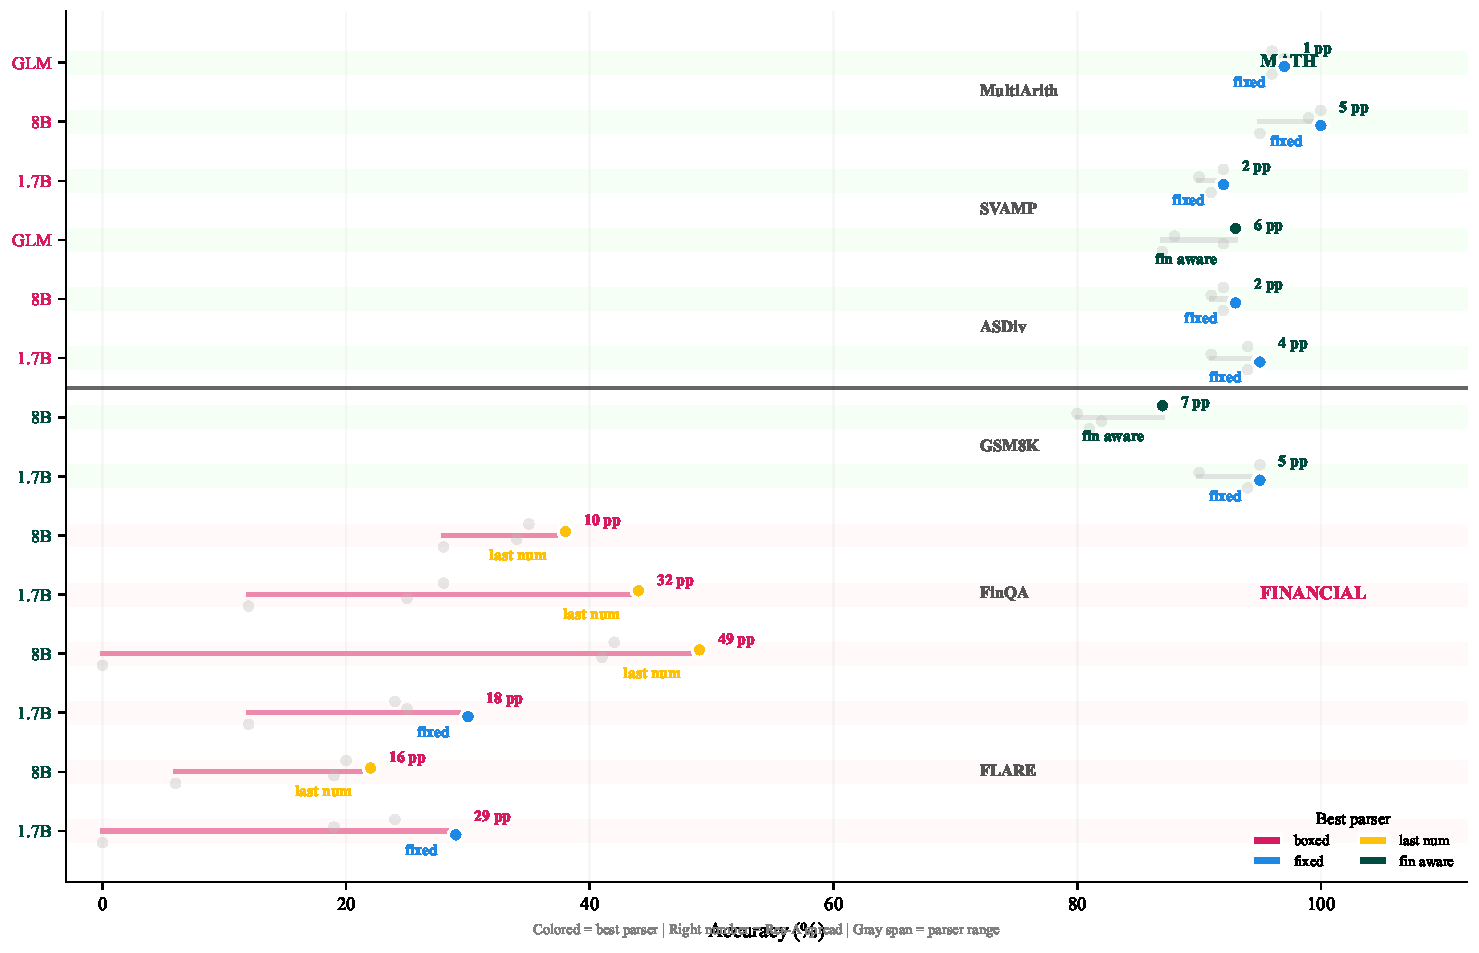
\includegraphics[width=\textwidth]{figures/figure2_best_parser.pdf}
    \caption{%
    Best parser varies by benchmark and model.
    Each row shows the accuracy range of four reasonable parsers (excluding \numparser{}) for one model--benchmark pair.
    The highlighted dot marks the best parser for that condition.
    The Res-A spread (right) measures the residual sensitivity among reasonable parsers.
    Math benchmarks (top) show tight agreement (1--7\,pp spread); financial benchmarks (bottom) show wide disagreement (10--39\,pp).
    Note that \texttt{last\_number} dominates FinQA while \texttt{fixed} dominates FLARE-FinQA---there is no single ``correct'' parser for financial evaluation.}
    \label{fig:best_parser}
\end{figure*}

% --- Figure 3: Res-A vs Res-B comparison ---
\begin{figure}[htb!]
    \centering
    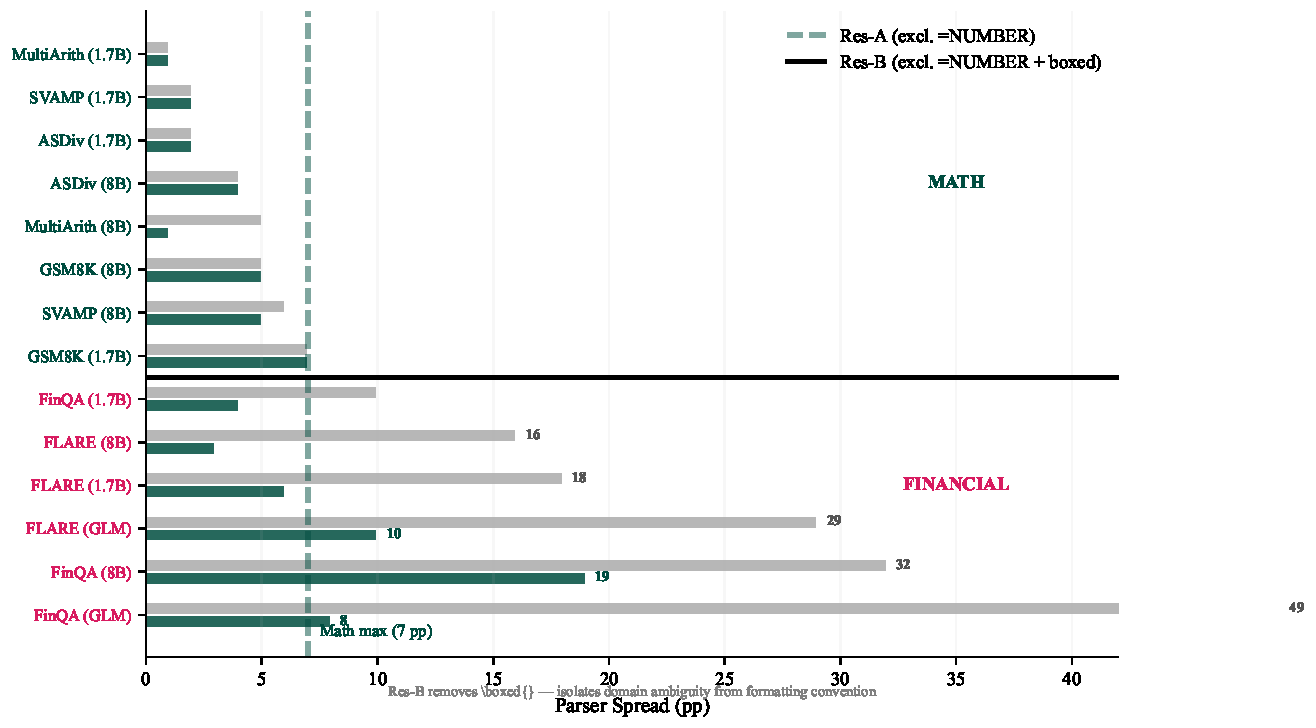
\includegraphics[width=\columnwidth]{figures/figure3_resA_resB.pdf}
    \caption{%
    Res-A versus Res-B: does including \boxedparser{} inflate residual sensitivity?
    Res-A (gray) excludes only \numparser{}; Res-B (green) excludes both \numparser{} and \boxedparser{}.
    The vertical dashed line marks the maximum Res-A value on math benchmarks (7\,pp).
    Financial benchmark spreads narrow under Res-B but remain elevated on the conditions with the largest effects (FinQA 8B/30B $\ge$ 20\,pp, FLARE GLM 10\,pp), confirming that domain-specific numeric conventions drive the residual gap beyond format-mismatch effects.
    Some financial conditions (FLARE 8B/30B) narrow to math-like levels, suggesting partial format-driven sensitivity.}
    \label{fig:resAB}
\end{figure}
